\documentclass{article}
\usepackage[utf8]{inputenc}
\usepackage[spanish]{babel}
\usepackage{listingsutf8}
\usepackage{xcolor}
\usepackage{pdfpages}
\usepackage{geometry}
% to install algorithm2e pckg: sudo apt-get install texlive-science
\usepackage[ruled, vlined, nofillcomment]{algorithm2e}
\usepackage{float}
%\usepackage{hyperref}
\usepackage{amsmath}
\usepackage{framed}

\geometry{
    a4paper,
    margin=1.2in
}

\title{75.29 - Teoría de Algoritmos I: Trabajo Práctico n. 3}
\author{
    \\\\\\\\
    \Large{Equipo Q:}\\
    Lavandeira, Lucas (\texttt{\#98042})\\\texttt{lucaslavandeira@gmail.com}\\
    \\
    Rozanec, Matias (\texttt{\#97404})\\\texttt{rozanecm@gmail.com}\\
    \\
    Sbruzzi, José (\texttt{\#97452})\\\texttt{jose.sbru@gmail.com}\\
    \\\\\\\\\\\\\\
}
\date{18.junio.2018}

\begin{document}
\maketitle
\begin{figure}[!htp]
    \centering
    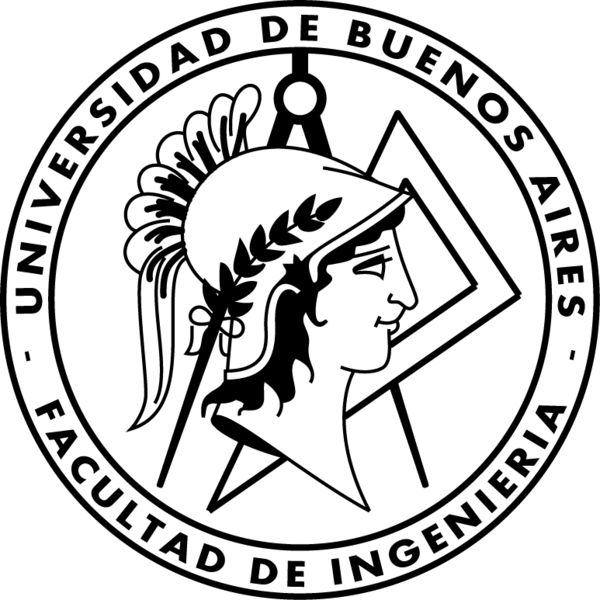
\includegraphics[scale=1]{res/fiuba_logo.png} 
\end{figure}
\begin{center}\normalsize{Facultad de Ingeniería, Universidad de Buenos Aires}\end{center}
\newpage

\tableofcontents
\newpage

% *** RESOLUCION ***
% Some settings for coding style
\lstset{
    basicstyle=\linespread{0.9}\ttfamily\footnotesize,
    frame=single,
    frameround=tttt,
    numbers=left,
    numberstyle=\tiny,
    linewidth=14cm,
    literate=
      {á}{{\'a}}1 {é}{{\'e}}1 {í}{{\'i}}1 {ó}{{\'o}}1 {ú}{{\'u}}1
      {Á}{{\'A}}1 {É}{{\'E}}1 {Í}{{\'I}}1 {Ó}{{\'O}}1 {Ú}{{\'U}}1
      {à}{{\`a}}1 {è}{{\`e}}1 {ì}{{\`i}}1 {ò}{{\`o}}1 {ù}{{\`u}}1
      {À}{{\`A}}1 {È}{{\'E}}1 {Ì}{{\`I}}1 {Ò}{{\`O}}1 {Ù}{{\`U}}1
      {ä}{{\"a}}1 {ë}{{\"e}}1 {ï}{{\"i}}1 {ö}{{\"o}}1 {ü}{{\"u}}1
      {Ä}{{\"A}}1 {Ë}{{\"E}}1 {Ï}{{\"I}}1 {Ö}{{\"O}}1 {Ü}{{\"U}}1
      {â}{{\^a}}1 {ê}{{\^e}}1 {î}{{\^i}}1 {ô}{{\^o}}1 {û}{{\^u}}1
      {Â}{{\^A}}1 {Ê}{{\^E}}1 {Î}{{\^I}}1 {Ô}{{\^O}}1 {Û}{{\^U}}1
      {œ}{{\oe}}1 {Œ}{{\OE}}1 {æ}{{\ae}}1 {Æ}{{\AE}}1 {ß}{{\ss}}1
      {ű}{{\H{u}}}1 {Ű}{{\H{U}}}1 {ő}{{\H{o}}}1 {Ő}{{\H{O}}}1
      {ç}{{\c c}}1 {Ç}{{\c C}}1 {ø}{{\o}}1 {å}{{\r a}}1 {Å}{{\r A}}1
      {€}{{\euro}}1 {£}{{\pounds}}1 {«}{{\guillemotleft}}1
      {»}{{\guillemotright}}1 {ñ}{{\~n}}1 {Ñ}{{\~N}}1 {¿}{{?`}}1
}



\part{Un juego de batalla naval}
\section{Instrucciones de ejecución}
En el directorio root del proyecto, correr \texttt{npm i} para instalar las 
dependendicas necesarias.\\
Para la ejecución propiamente dicha, correr el comando \texttt{npm start}
seguido de los siguientes argumentos:
\begin{itemize}
        \item ruta al archivo que contiene la información del juego
        \item selección de estrategia: \texttt{greedo} o 
            \texttt{dinamico} 
        \item cantidad de lanzaderas 
        \item \textbf{opcional} \texttt{true} o \texttt{false} de acuerdo a si se 
            desea utilizar posiciones iniciales de los barcos distintas a 0.
            Default: \texttt{false}.
\end{itemize}
\section{Dinamico}
\subsection{Explicación del algoritmo}

\begin{algorithm}
\caption{mejoresPartidas(t,d)}
\KwData{Cantidad de turnos $t$ que demoran las partidas retornadas y disparos $d$ que se dispararán a continuación}
\KwResult{Partidas con menor cantidad de puntos obtenidas}
    $d \leftarrow \text{siguiente disparo}$ \\
    $t \leftarrow \text{turno actual}$ \\
    \If{$t=0$}{
        \KwRet{partida inicial sin disparos}
    }\Else{
        A $\leftarrow \bigcup_{d' \in D}$ mejoresPartidas$(t-1,d')$ \\
        A $\leftarrow$ conDisparo($d$,A) \\
        $p^* \leftarrow max_{a \in A}\left \{puntaje(a)\right \}$ \\
        $A^* \leftarrow \{ a \in A / puntaje(a)=p^*\}$ \\
        \KwRet{$A^*$}
    }
\end{algorithm}

El algoritmo pretende devolver la lista de las mejores partidas posibles que se resuelvan en t turnos y que terminen con el disparo d, sin embargo, no lo logra. Devuelve las mejores partidas posibles al aplicarles el disparo d a cada una de las mejores partidas posibles en t-1 turnos.

En la implementación javascript, los hiperparámetros del algoritmo (es decir, el tablero, la cantidad de lanzaderas, la cantidad de barcos y los puntos de vida de cada uno) también se pasan como argumentos.

\subsubsection{Calidad de heurística de Dinámico}

Dinamico no conforma un algoritmo de resolución de la situación planteada, sino una heurística. Esto se demuestra por medio del siguiente contraejemplo.

\begin{center}
\begin{tabular}{ c | c c c c c c c c c c c c c}
Hay una sola lanzadera. \\
\hline
V\_i & t1 & t2 & t3 & t4 & t5 & t6 & t7 & t8 & t9 & t10 & t11 & t12 & t13 \\
\hline
10    &  9 &  1 &  1 &  1 &  1 &  1 & 1 &  1 &  1 &  1 &  1 & 1  & 10 \\
1     &  1 &  1 &  1 &  1 &  1 &  1 & 1 &  1 &  1 &  1 &  1 & 1  & 10
\end{tabular}
\end{center}

En la solución mínima, el barco de vida 10 recibe un disparo en el primer turno, aprovechándose de esta forma el gran daño que puede recibir; y el puntaje alcanzado es 5. Sin embargo, debido a que Dinámico es una heurística que aplica un criterio de greedy para determinar la mejor decisión por turno, determina que la mejor decisión para el primer turno es la que lleve a un mejor puntaje, es decir, disparar al barco de salud 1 primero y al de salud 10 después. Así, el puntaje mínimo alcanzado por Dinámico será 11.

\subsubsection{Complejidad temporal del algoritmo}

El algoritmo Dinamico es memoizado. Como sus únicos parámetros son t y d, su complejidad temporal será lineal respecto de los valores que puede tomar cada uno de sus parámetros. En memoria, se generará una tabla como la siguiente:
\begin{center}
\begin{tabular}{c | c c c c}
turno & disparo posible 1 & disparo posible 2 & disparo posible 3 & ... \\
t\_0 & & & & \\
t\_1 & & & & \\
t\_2 & & & & \\
t\_3 & & & & \\
t\_4 & & & & \\
t\_5 & & & & \\
... & & & &
\end{tabular}
\end{center}
El costo añadido de computar la solución en cada "casilla" de la tabla es lineal al costo de obtener el puntaje de cada partida alternativa, y por lo tanto a la cantidad de partidas alternativas. Por otro lado, el costo de computar el puntaje de cada partida alternativa es lineal con la cantidad de barcos (ya que es necesario determinar si cada uno de ellos está vivo en la misma). Así, el costo del algoritmo memoizado para resolver $mejoresPartidas(t,d)=O(t*disparos posibles*costo de cada casillero)=O(t*disparos posibles*disparos posibles*costo de obtener puntaje de una partida)=O(t*disparos posibles*disparos posibles*barcos)=O(t*disparos posibles^2*barcos)$.

\subsection{Condiciones para que Dinámico sea óptimo}
Dinámico será óptimo cuando la mejor decisión posible en cada turno sea la que más barcos mate en ese turno. Esto sólo puede darse cuando las vulnerabilidades relacionadas a cada barco solamente ascienden a lo largo de la partida, cuando el tablero no es "rotatorio", tal como fue el planteo dado, es necesario asegurar también que ninguna partida dura tantos turnos como columnas del tablero. A continuación se demuestra esta afirmación para un tablero infinito, sin repeticiones.

\subsection{Planteo matemático de la hipótesis y demostración}

\subsubsection{Conceptos necesarios para expresar la hipótesis y la prueba}

Sea $v(t,b)$ la vulnerabilidad del barco $t$ en el turno $b$, con $t\geq0$ y $1\geq b \geq B$, siendo $B$ la cantidad de barcos.
Sea $d(t,b)$ una función tal que

\[
    d(t,b)=
    \begin{cases}
        1 & \text{si se dispara al barco $b$ en el turno $t$} \\
        0 & \text{en otro caso}
    \end{cases}
\]
Y sea $D$ el conjunto de todos los disparos $d$ que cumplen que:
$$ \sum_{b=1}^{B} d(t,b) = L  \forall t \geq 0 $$

Sea $h_{d,v} (t,b)$ una función que representa la salud del barco $b$ en el turno $t$, al usar los disparos $d$ y las vulnerabilidades $v$:
\[
    h_{d,v}(t,b)=
    \begin{cases}
        h(t-1,b)-v(t,b) \cdot d(t,b) & \text{si $t>0$} \\
        V_b & \text{si t=0}
    \end{cases}
\]
Siendo $V_b$ la salud inicial de cada barco. Sea $H_{d,v}(b,t)$ una función que indica si el barco $b$ vive en el turno $t$, usando los disparos $d$ y las vulnerabilidades $v$.
\[
    H_{d,v}(t,b)=
    \begin{cases}
        1 & \text{si $h_{d,v}(t,b)>0$} \\
        0 & \text{en caso contrario}
    \end{cases}
\]

Y sea también $H_{d,v}(t)$ tal que: $$H_{d,v}(t)=\sum_{b=1}^{B} H_{d,v}(t,b)$$

Sea la función $G(d,v,t)$ que indica si en el turno $t$, el disparo $d$ representa una formado por medio de la estrategia greedy, que consiste en elegir el disparo que destruya más barcos:
\[
    G(d,v,t)=
    \begin{cases}
        1 & \text{si $h_{d,v}(t)=min_{d' \in D} \left \{ H_{d',v}(t) \right \} $} \\
        0 & \text{si no}
    \end{cases}
\]

Sea la función $G*(d,v,t)$ que representa si los disparos de todos los turnos hasta $t$ fueron greedy:
\[
    G^*(d,v,t)=
    \begin{cases}
        G(d,v,t) \cdot G^*(d,v,t-1) & \text{si $T>0$} \\
        1 & \text{si $T=0$}
    \end{cases}
\]

Sea la función $P_{d,v}(t)$ la cantidad de puntos acumulados hastael turno $t$ al usar el disparo $d$ y las vulnerabilidades $v$:
\[
    P_{d,v}(t)=
    \begin{cases}
        H_{d,v}(t) + P_{d,v}(t-1) & \text{si $t>0$} \\
        0 & \text{si $t=0$}
    \end{cases}
\]


\subsubsection{Hipótesis}
\begin{framed}
Para cualquier $T$ natural mayor a 0 se cumple que: \newline
Dado $v$ tal que: 
$$ v(t+1,b) 
\geq 
v(t,b) \forall 0 \leq t \leq T, 1 \leq b \leq B $$
Y dado $d$ tal que: $$G^*(d,v,T)=1$$
Entonces: $$P_{d,v}(T)=min_{d' \in D} \left \{ P_{d',v}(T) \right \}$$
\end{framed}

\subsubsection{Demostración: caso base}
Para $T=0$ la hipótesis es verdadera porque $P_{d,v}(T)=0 \forall d,v$.


\subsubsection{Planteo del caso inductivo}
Para $T > 0$, tenemos que se cumple para $T-1$ que:
\begin{framed}
Dado $v$ tal que: $$ v(t+1,b) \geq v(t,b) \forall 0 \leq t \leq T-1, 1 \leq b \leq B $$
Y dado $d$ tal que: $$G^*(d,v,T-1)=1$$
Entonces: $$P_{d,v}(T-1)=min_{d' \in D} \left \{ P_{d',v}(T-1) \right \}$$
\end{framed}
A partir de esa proposición, queremos probar que teniendo:
\begin{framed}
Dado $v$ tal que: $$ v(t+1,b) \geq v(t,b) \forall 0 \leq t \leq T, 1 \leq b \leq B $$
Y dado $d$ tal que: $$G^*(d,v,T)=1$$
\end{framed}
Podemos concluir que: $$P_{d,v}(T)=min_{d' \in D} \left \{ P_{d',v}(T) \right \}$$

\subsubsection{Demostración del caso inductivo}
Por la definición de $P$: $$P_{d,v}(T)=H_{d,v}(T)+P_{d,v}(T-1)$$
Por la hipótesis inductiva, que afirma que $P_{d,v}(T-1)=min_{d^* \in D}\left \{ P_{d^*,v}(T-1) \right \}$ podemos definir que:
$$P_{d,v}(T)=H_{d,v}(T)+min_{d^* \in D}\left \{ P_{d^*,v}(T-1) \right \}$$

Debido a que: $$G^*(d,v,T)=1 \Rightarrow G(d,v,T)=1 \Rightarrow H_{d,v}(T)=min_{d' \in D} \left \{ H_{d',v}(T) \right \}$$
Podemos concluir, combinando estas últimas dos proposiciones, que:
$$P_{d,v}(T)=min_{d' \in D} \left \{ H_{d',v}(T) \right \}+min_{d^* \in D}\left \{ P_{d^*,v}(T-1) \right \}$$

Una manera alternativa de definir $P_{d,v}(t)$ es:$$P_{d,v}(t)=\sum_{i=1}^{t} H_{d,v}(i)$$

Agregando esta definición a la proposición anterior tenemos que:

$$P_{d,v}(T)=min_{d' \in D} \left \{ H_{d',v}(T) \right \}+min_{d^* \in D}\left \{ \sum_{i=1}^{T-1} H_{d^*,v}(i) \right \}$$
Debido a que los disparos $d$ en cada uno de los turnos son independientes, y la minimización tiene en cuenta sólo la efectividad de cada turno:
$$P_{d,v}(T)=min_{d' \in D} \left \{ H_{d',v}(T) \right \}+\sum_{i=1}^{T-1} min_{d^* \in D}\left \{  H_{d^*,v}(i) \right \}$$

$$P_{d,v}(T)=\sum_{i=1}^{T} min_{d^* \in D}\left \{  H_{d^*,v}(i) \right \}$$

Teniendo en cuenta la independencia de los disparos en cada uno de los turnos citada anteriormente, consecuencia de la condición impuesta sobre $v$, que implica que cualquier barco que podría haber sido destruído en cierto turno puede ser destruído en el siguiente, podemos concluir que:
$$P_{d,v}(T)=min_{d'' \in D}\left \{ \sum_{i=1}^{T} H_{d'',v}(i) \right \}$$
Lo cual concluye la demostración.

\section{Greedo}

\subsection{Explicación del algoritmo}

\begin{algorithm}
\caption{obtenerMejor(p)}
\KwData{Partida inicial a mejorar $p$}
\KwResult{La mejor partida que puede obtener el algoritmo}
    $p \leftarrow \text{Partida a mejorar}$ \\
    \If{$barcosVivos(p)=0$}{
        \KwRet{$p$}
    }\Else{
        $D' \leftarrow \{ d \in D / \text{ $d$ impacta barcos vivos de $p$ }\}$ \\
        $P \leftarrow$ conDisparo($D'$,$p$)\\
        $p^* \leftarrow$ una de las partidas con el menor puntaje posible de $P$ \\
        \KwRet{ $obtenerMejor(p^*)$ }
    }
\end{algorithm}

En el caso del algoritmo Greedy, para elegir el mejor disparo se utilizó una heurística más efectiva que para la solución dinámica. Greedo evalúa según el mejor puntaje posible a cada paso. Este puntaje se obtiene suponiendo que en todos los turnos siguientes se dispone de tantas lanzaderas como barcos. Así, al intentar maximizar el mejor puntaje posible en vez del puntaje actual, Greedo no prioriza el disparo que más barcos mate sino el disparo que haga que la solución empeore lo menos posible.

Para ponerlo en términos más sencillos, Greedo se pregunta, para cada barco \textit{Cuánto pierdo si no te disparo?} y evaluando eso define qué movimiento hacer a continuación.

\subsection{Calidad de heurística de Greedo}
A continuación se presenta un caso en el que el algoritmo Greedy falla.

Hay una sola lanzadera. \\
\begin{center}
\begin{tabular}{ c | c c c c c c c c c c c c c}
\hline
V\_i & t1 & t2 & t3 & t4 & t5 & t6 & t7 & t8 & t9 & t10 & t11 & t12 & t13 \\
\hline
15    &  5 &  5 &  10 &  0.1 &  0.1 &  0.1 & 0.1 &  0.1 &  0.1 &  0.1 &  0.1 & 0.1  & 0.1 \\
10    &  1 &  0 &  10 &  1 &  1 &  1 & 1 &  1 &  1 &  1 &  1 & 1  & 1
\end{tabular}
\end{center}

En este caso, el algoritmo puede tomar dos decisiones distintas respecto del primer disparo: o bien dispararle al barco de salud 15 o bien al de salud 10. Ambas decisiones tienen la misma penalización, debido a que la misma está definida por el puntaje que se alcanzaría si se pudiera disparar 2 veces por turno y, al comenzar, ambos barcos serían dstruídos en la columna t3 según esta aproximación. La decisión desemboca en una de dos situaciones:

Disparando inicialmente al barco de vida 15. Hay una sola lanzadera. \\
\begin{center}
\begin{tabular}{ c | c c c c c c c c c c c}
\hline
V\_i &   t3 & t4 & t5 & t6 & t7 & t8 & t9 & t10 & t11 & t12 & t13 \\
\hline
5     &  10 &  0.1 &  0.1 &  0.1 & 0.1 &  0.1 &  0.1 &  0.1 &  0.1 & 0.1  & 0.1 \\
10    &  10 &  1 &  1 &  1 & 1 &  1 &  1 &  1 &  1 & 1  & 1
\end{tabular}
\end{center}

A partir de aquí, el algoritmo decide disparar al barco que ahora tiene vida 5, con lo cual, a partir de este turno, se alcanza un puntaje de 10 puntos. La alternativa es disparar al barco de vida 10, lo cual llevaría a un puntaje de 50 puntos.

Disparando inicialmente al barco de vida 10. Hay una sola lanzadera. \\
\begin{center}
\begin{tabular}{ c | c c c c c c c c c c c}
\hline
V\_i &   t3 & t4 & t5 & t6 & t7 & t8 & t9 & t10 & t11 & t12 & t13 \\
\hline
10    &  10 &  0.1 &  0.1 &  0.1 & 0.1 &  0.1 &  0.1 &  0.1 &  0.1 & 0.1  & 0.1 \\
9     &  10 &  1 &  1 &  1 & 1 &  1 &  1 &  1 &  1 & 1  & 1
\end{tabular}
\end{center}

A partir de aquí, el algoritmo decide disparar al barco que ahora tiene vida 10 (de lo contrarío obtendría un puntaje de 100), y alcanza una penalización de 9.\\

Así, vemos que el algoritmo puede alcanzar situaciones subóptimas cuando encuentra que debería destruir más barcos de los que le es posible en la misma columna. El algoritmo Baco, codificado de forma similar a Greedo, postpone estas decisiones, devolviendo a cada paso las mejores soluciones posibles. Se incluyó en el código del trabajo práctico.

\subsection{Complejidad temporal del algoritmo Greedo}
El algoritmo Greedo ejecuta una única llamada recursiva, que concluye cuando el algoritmo destruye todos los barcos. Así, tal llamada recursiva implica una complejidad temporal de $O(\text{ejecucion} \cdot \text{turnosMaximos})$.

El tiempo de ejecución del algoritmo en sí es lineal con el tiempo de ejecución del algoritmo que calcula el mejor puntaje posible de una partida y la cantidad de configuraciones de disparos posibles: $O(\text{calculo mejor puntaje posible} \cdot \text{disparos posibles} \cdot \text{turnosMaximos})$.

El cálculo del mejor puntaje posible es lineal con la cantidad de barcos y con el tiempo de ejecución del algoritmo que descubre la supervivencia mínima de cada barco:$O(\text{cálculo supervivencia mínima} \cdot \text{barcos}  \cdot \text{disparos posibles} \cdot \text{turnosMaximos})$.

El algoritmo que descubre la supervivencia mínima de cada barco tiene una complejidad temporal que depende totalmente del problema: Se inicializa una variable con la salud del barco y se recorren las columnas avanzando y restando la vulnerabilidad correspondiente del acumulador hasta que el mismo se torne 0. Es posible escribir este algoritmo de forma que sea lineal con la cantidad de casilleros de la fila del barco. A continuación se detalla el pseudocódigo para lo mismo:

\begin{algorithm}
\caption{supervivencia(v,h)}
    $v \leftarrow \text{array de vulnerabilidades de la fila}$ \\
    $h \leftarrow \text{Salud inicial del barco analizado}$ \\
    
    
    $T \leftarrow \text{Suma de todos los valores de } v$ \\
    $vueltas \leftarrow \lfloor h / T \rfloor $ \\
    $i \leftarrow vueltas \cdot len(v)$ \\
    $h \leftarrow h-vueltas \cdot T$ \\
    
    \While{$h > 0$}{
        $i \leftarrow i+1$\\
        $h \leftarrow h-v_i$\\
    }
    \KwRet{$i$}
    
    
\end{algorithm}

Por lo tanto, el algoritmo tiene la complejidad temporal:
$$O(\text{columnas del tablero} \cdot \text{barcos}  \cdot \text{disparos posibles} \cdot \text{turnosMaximos})$$


\subsection{Condiciones para que Greedo sea óptimo}
Greedo es óptimo cuando no se da la necesidad de tomar decisiones alternativas, es decir, cuando hay una única solución mejor. 

El menor puntaje estimado siempre será mayor al puntaje de la solución real, siempre y cuando la cantidad de barcos vivos sea mayor a la cantidad de lanzaderas. De lo contrario, estos puntajes serán iguales. Así, el juego nunca puede terminar con un puntaje menor al mínimo estimado. El algoritmo Baco descarta unicamente las decisiones que perjudican esta cota inferior. Sin embargo, la misma crece a lo largo de la ejecución del programa, hasta que coinciden la cota inferior y el puntaje encontrado. Debido a esto, es razonable pensar que Baco llega al óptimo. Esta afirmación no se demuestra sino que se deja como razonable.

Greedo, por otro lado, sí descarta decisiones que tienen la menor cota, con lo cual, puede descartar una "rama" de decisiones que lleve a la solución óptima, la cual sí alcanzaría Baco. En el código se incluye el algoritmo Dinámico Jr., que aplica la heurística de Greedo al esquema de Dinamico. Es posible que ese algoritmo sí pueda alcanzar el óptimo en tiempo polinómico.

\section{Posicionamiento inicial de barcos}
La esencia del algoritmo se basa en analizar, por cada uno de los barcos, cuál 
será el casillero de inicio que le brindará la mayor cantidad de puntos. Esto 
se logra haciendo avanzar al barco un casillero hacia adelante y restándole en 
cada paso la cantidad de vida correspondiente, hasta que el barco es destruido.
La posición inicial óptima será la que le brinde al barco la mayor cantidad de 
posiciones avanzadas. La complejidad para el cálculo inicial de cada uno de los
barcos es entonces linealmente proporcional a la cantidad de columnas. 

\newpage
\part{Parte 2: Sabotaje!}

\subsection{Análisis preliminar y consideraciones previas}
El problema planteado implica un conocimiento de redes de flujo. Una definición con la que trabajaremos es la siguiente: se entiende como red de flujo a un grafo dirigido con aristas pesadas. Llamamos al peso de cada arista la capacidad entre los dos vértices que conecta. Las redes de flujo cumplen las condiciones:
\begin{itemize}
    \item Existe un único vértice con únicamente aristas salientes a él, sin aristas entrantes, llamado fuente.
    \item Existe un único vértice con únicamente aristas entrantes a él, sin aristas salientes, llamado sumidero.
    \item Todos los demás vértices cumplen la condición de que la capcidad entrante, es decir, la sumatoria de todas sus aristas que terminan en este vértice, es igual a la capcidad saliente, la sumatoria de todas las aristas con fuente en este vértice.
\end{itemize}

La última condición implica una conservación de la capacidad: en la red, todos los nodos intermedios entre la fuente y el sumidero tienen una capacidad neta nula, solo transportan capacidad entre las puntas, sin crear o destruir capacidad adicional.

Las redes de flujo modelan problemas en donde, valga la redundancia, fluye una cantidad apreciable de un bien sobre ciertas vías (los ejes o aristas), en donde cada vértice marca una intersección donde se puede redirigir la dirección del flujo. Las aplicaciones más comunes es en líquidos en cañerías en un problema de hidráulica, corriente eléctrica en un circuito, o el tránsito en un sistema de autovías, entre otros.
 
Definimos flujo de un eje como la cantidad de ese valor modelado (corriente, líquido, tránsito), que está circulando actualmente entre los nodos determinados. Este valor, por supuesto, debe ser menor a la capacidad total de ese eje, y también debe cumplir la condición de conservación: el flujo entrante a un nodo es igual al saliente.

El cuello de botella, \textit{bottleneck}, de un camino entre fuente y sumidero es la capacidad mínima de todos los ejes del camino. Este valor es el flujo máximo que puede llegar a circular por ese camino, debido a la condición anterior de que el flujo no puede ser mayor a las capacidades de los ejes por el que pasa.

\begin{figure}[H]
    \centering
    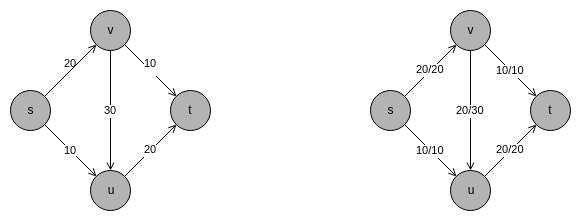
\includegraphics[scale=0.5]{res/flow_network.png}
    \caption{Red de flujo con capacidades totales y con flujo/capacidad total}
\end{figure}

Leyendo el enunciado se toman varias suposiciones. La más importante es que la red que tenemos que proteger es una red de flujo de manera tal que cumpla con la definición dada anteriormente. Lo segundo es la interpretación de "los saboteadores quieren hacer el máximo daño posible" del enunciado. Se entiende que los saboteadores actúan de manera completamente óptima: Primero sabotearán el eje más importante de la red (a definir más adelante), y luego, el segundo más importante, que será el eje más importante de la red de flujo resultante al tener inoperante el primer eje. Dicho de otra manera, los saboteadores atacan como segundo eje al que sería más importante en una red de flujo que no contenga al primer eje saboteado.

No está de más aclarar también que la solución implementada es óptima y termina con el orden determinado únicamente cuando las capacidades de los ejes son números enteros. 

\subsection{Algoritmo propuesto}

El problema se resume en determinar las dos aristas más importantes de la red. Es sencillo de ver que si encontramos el flujo máximo que puede pasar por nuestra red, las aristas más importantes serán las que mayor flujo pasen por ellas. El algoritmo a proponer se resume a este concepto, hallamos el flujo máximo de la red, y luego iteramos sobre todas las aristas de la red y detectamos las de mayor flujo. El flujo máximo se calcula por el algoritmo de Ford Fulkerson, con la búsqueda de caminos fuente-sumidero usando DFS. 

El algoritmo implementado es óptimo gracias a la garantía de que el flujo máximo encontrado es óptimo, Ford Fulkerson determina la mayor cantidad de flujo pasable por la red. Sabiendo que los flujos son óptimos, el resultado de iterar sobre ellos devolverá las aristas más importantes también será óptimo.

\begin{algorithm}
    \KwData{$G$: red de flujo a determinar vulnerabilidades, $n$: cantidad de ejes a proteger}
    \KwResult{$vul$: lista de ejes a proteger}
    \BlankLine

    $R$ $\leftarrow$ FordFulkerson(G); // Grafo residual
    
    vul $\leftarrow$ [];

    \While{$vul.length < n$}{
        \ForEach{$e \in E(R)$}{
            \If{$vul.length < n$}{
                vul.append(e);
            } \ElseIf{$e.flow > min(vul)$}{
                vul.remove(min(vul));

                vul.append(e);
            }
        }
    }
    return $vul$;

    \caption{Pseudocódigo del algoritmo propuesto}
\end{algorithm}

La complejidad del algoritmo está acotada por Ford Fulkerson, de orden $O(mC)$, siendo $m$ la cantidad de vértices de la red, y $C$ la capacidad saliente de la fuente. El hallado de los ejes más importantes de la red es una búsqueda lineal sobre las mismas, $O(n) = O(2m) = O(m)$. Se podría ver como una reducción sobre Ford Fulkerson: se está usando el algoritmo de flujo máximo como una caja negra, y simplemente iterando sobre sus resultados (transformación de valores de salida) para determinar la solución a nuestro problema.

La complejidad es calculada de esta manera gracias a la suposición de que las capacidades son valores enteros. El algoritmo de Ford Fulkerson utiliza esta suposición para dar su propia cota de complejidad. De ser las capacidades un valor fraccionario, ni siquiera se podría garantizar la terminación del algoritmo, debido a que en el peor caso Ford Fulkerson podría llegar a aumentar su flujo de a cantidades arbitrariamente pequeñas hasta llegar al máximo.

Analizando los flujos máximos antes y después del sabotaje podemos apreciar que el flujo no necesariamente difiere en la cantidad exacta de los flujos de las aristas saboteadas. Si borramos esas aristas, el flujo puede ser redirigido y tomar una dirección con capacidad disponible que antes no hacía porque simplemente no era conveniente.

\subsection{Extensión con varias fuentes y sumideros}

Se plantea la situación del mismo problema, pero ahora con una red que tenga varios nodos fuente y sumidero. Se puede ver de manera sencilla que una red con varias fuentes y sumideros es una composición de varias redes individuales de una única fuente y único sumidero.

Comencemos con una red de 1 fuente, 1 sumidero. Esta red ya fue definida anteriormente, en particular restaltamos la propiedad de conservación del flujo en cada nodo interior. Agregar una fuente y un sumidero nuevo implicaría agregar esos dos nodos, más los ejes que transporten flujos entre ellos, agregando también nodos adicionales si se quiere, pero también podrían utilizarse los mismos nodos de la red original. Agregar un eje acá puede implicar simplemente aumentar la capacidad máxima del eje entre dos nodos, no necesariamente haya que agregar una nueva arista al grafo que representa la red.

De esta manera se puede ver que para cualquier fuente de flujo existe al menos un camino desde una fuente a algún sumidero. La idea principal para resolver este caso, entonces, es descomponer a la red de múltiples fuentes - sumideros en caminos o subgrafos en donde haya una correspondencia 1:1, y luego aplicar el algoritmo de flujo máximo sobre cada uno, y sumar los resultados. Esta suma de flujos es el flujo máximo de la red original propuesta. Desde allí basta con detectar los dos ejes de mayor flujo.

La descomposición puede resultar difícil de plantear como un algoritmo pero basta modificar la Implementación actual que busca caminos entre la única fuente y el único sumidero a buscar caminos desde \textit{cualquier} fuente hasta \textit{cualquier} sumidero, que es equivalente a la descomposición, por lo menos para el propósito que se estaría usando en este caso. El orden del algoritmo no es modificado, sigue estando acotado por la cantidad de nodos, y la capacidad mínima de la red, debido al uso de Ford-Fulkerson internamente.

\subsection{Implementación}

Se implementó el algoritmo propuesto (junto con Ford Fulkerson) en Nodejs. Para correr el código, asegurarse de contar con una versión de Node $>=$ 8.0, correr \textit{npm i}, y luego \textit{npm start}.

\newpage
\part{Anexo: Correcciones de Sabotaje!}
La suposición que se toma es que KAOS quiere disminuir el flujo lo más posible.
\begin{algorithm}
    \KwData{$G$: red de flujo a determinar vulnerabilidades, $n$: cantidad de ejes a proteger}
    \KwResult{lista de ejes a proteger}
    \BlankLine

    $R$ $\leftarrow$ FordFulkerson($G$) // Grafo residual \\
    //las pertenecientes al corte mínimo \\
    $aristasCorte$ $\leftarrow$ obtenerAristasCorte($R$) \\
    $primeraVictima$ $\leftarrow$ $e$ $\in$ $aristasCorte$ / $capacidad_e$ = $max_{e \in aristasCorte}$ \{ $capacidad_e$ \} \\
    $primerFlujo$ $\leftarrow$ flujo(R)$-$ $capacidad_{primeraVictima}$ \\
    $ataques$ $\leftarrow$ \{($primerFlujo$,$atacada$)\}\\
    $victima$ $\leftarrow$ $primeraVictima$ \\
    \BlankLine
    $flujoNuevo$ $\leftarrow$ 0\\
    \While{$flujoNuevo < $ max\{ f / (f,v) $\in$ ataques \}}{
        $R$ $\leftarrow$ $R$.cambiarCapacidad($victima$,$\infty$)\\
        //cambiarCapacidad continúa la ejecución de Ford Fulkerson\\
        aristasCorte $\leftarrow$ obtenerAristasCorte($R$)\\
        $victima$ $\leftarrow$  $e$ $\in$ $aristasCorte$ / $capacidad_e$ = $max_{e \in aristasCorte}$ \{ $capacidad_e$ \}\\
        $flujoNuevo$ $\leftarrow$ flujo(R) $-$ $capacidad_{victima}$\\

        \BlankLine

        $ataques$ $\leftarrow$ $ataques$ $\cup$ \{ (flujo,victima) \} \\

        \BlankLine
        \If{$|ataques|$ $>$ 2}{
            ataques $\leftarrow$ los dos (f,v) $\in$ $ataques$ con menor f \\
        }
    }
    \BlankLine
    return los dos (f,v) $\in$ $ataques$ con menor f \\

    \caption{Pseudocódigo del algoritmo propuesto}
\end{algorithm}
\subsection{Explicacion del algoritmo propuesto}
La fundamentación principal del algoritmo es el llamado \textit{max flow-min cut theorem}, enunciado en ``Algorithm Design'' de Kleinberg y Tardos como la afirmación 7.9. Este teorema establece que el flujo máximo es igual a la suma de las capacidades de las aristas del corte mínimo. Así, removiendo una arista de tal corte nos aseguramos que la capacidad del corte mínimo disminuye, y por lo tanto también el flujo máximo de la red.\\
Se elige remover, en cada caso, la arista del corte mínimo con mayor capacidad. Sin embargo, remover esta arista no asegura que el flujo decaiga lo más posible, ya que podría existir un corte que -sin ser el mínimo- pueda tener todavía menor capacidad al remover la arista de mayor capacidad que posee. El algoritmo construído intenta apalear esta situación averiguando el menor corte mínimo que sea mayor al analizado: imposibilita que el corte analizado sea mínimo asignando una capacidad infinita a la arista atacada, y luego continúa la ejecución de Ford-Fulkerson, para luego encontrar el siguiente corte mínimo. Se especula que el siguiente corte mínimo no sea demasiado mayor al encontrado antes, y se vuelve a proceder como antes, con la esperanza de que la nueva remoción sea mejor -o no demasiado peor- respecto de la anterior.\\
Se procede de esta manera de forma de obtener al menos dos soluciones. Sin embargo, si se encuentra que la siguiente solución es mejor, se continúan procesando más soluciones, con la esperanza de mejorar más a cada iteración.\\

\subsection{Naturaleza de heurística del algoritmo construído}
El algoritmo construído no descubre las aristas que causan la mayor disminución del flujo, como muestra el siguiente ejemplo:
\begin{figure}[H]
    \centering
    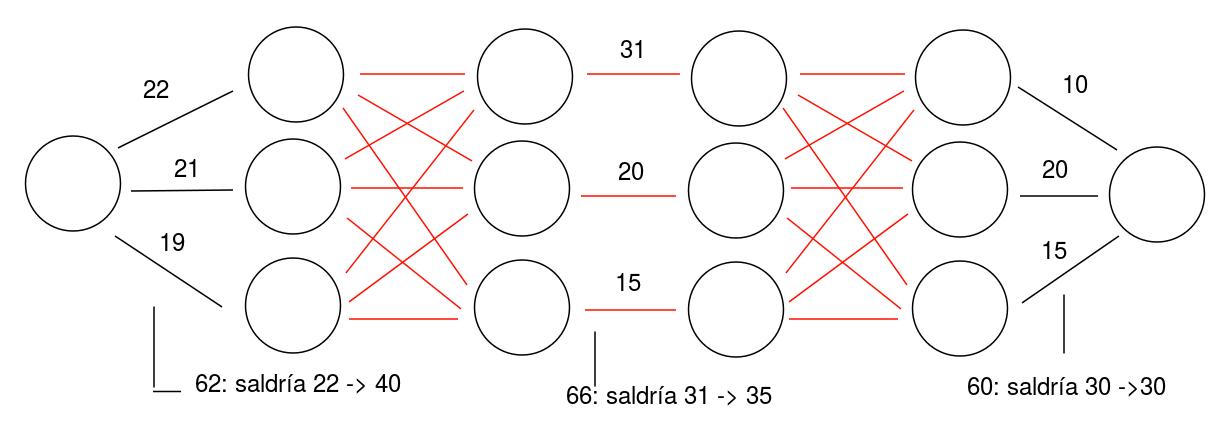
\includegraphics[scale=0.3]{res/contraejemplo.png}
    \caption{Contraejemplo}
\end{figure}
En este caso, el algoritmo primero eliminaría el vértice de valor 30, y luego, en vez a de priorizar el corte de capacidad 66, que llevaría a un flujo máximo de 35 al remover la arista correspondiente, prioriza el corte de capacidad 62, que lleva a uno de 40.

\subsection{Complejidad de la ejecución del algoritmo}
En el caso de que el algoritmo encuentre cada vez mejores aristas para remover, el ciclo terminará con la solución de flujo infinito, es decir, hará infinitas las capacidades de todas las aristas. Como el infinito es mayor que cualquier mínimo corte que se encuentre, esta es la última situación analizada posible. En este caso, itera tantas veces como aristas tenga el grafo.\\

Kleinberg-Tardos demuestran que en cada ciclo del algoritmo Ford Fulkerson, el flujo aumenta, y que aumenta como mínimo en una unidad (afirmaciones 7.2 y 7.3), así, establecen que el ciclo del algoritmo en el que se aumentan los flujos se ejecutará al menos C veces, siendo C una cota del flujo máximo. Kleinberg y Tardos acotan el flujo máximo con C igual a la suma de las capacidades salientes de la fuente.\\
Aquí pretendemos extender la cota temporal del algoritmo Ford-Fulkerson a redes de flujo con grafos con capacidades infinitas. En este caso, el flujo máximo o bien es infinito (en el caso de que exista un augmenting path conformado de aristas que sólo tienen capacidad infinita), o bien es un entero (si no existe tal augmenting path). Si el flujo máximo es un entero, debe ser menor o igual a la suma de todas las capacidades no infinitas de las aristas del grafo, ya que el corte mínimo debe estar conformado por aristas de capacidad entera (como mucho, todas). Si el flujo es infinito, es natural pensar que se encontrará en como mucho un path augmentation más que cualquier flujo entero. Por lo tanto, el algoritmo Ford-Fulkerson con capacidades infinitas tomará como mucho $K+1$ iteraciones, siendo $K$ la suma de las capacidades no infinitas.\\
Ahora pretendemos acotar temporalmente el algoritmo propuesto. Una primera cota es $O(m^{2K})$, es decir, la ejecución de Ford-Fulkerson $m$ veces. Sin embargo, como el algoritmo no se inicia de nuevo, sino que se continúa en cada ciclo, la cantidad de veces que se ejecutarán path augmentations será $m+K$, con lo cual tendremos una cota de $O(m*(m+K))$. Como $K\geq m$ (debido a que partimos de un grafo con capacidades finitas y enteras), tendremos la cota $O(m*K)$.\\

\textbf{Afirmación} La cantidad de veces que se ejecutan \textit{path augmentations} en nuestro algoritmo será como mucho $m+K+1$.\\

\textbf{Demostración} En cada ejecución del ciclo exterior de nuestro algoritmo, el flujo no disminuye, es decir, o bien aumenta, o bien permanece constante. Sea el aumento de flujo en el ciclo $i$ $\delta_i$, siendo $\delta_i \geq 0$, con $\delta_0$ el flujo inicial. En nuestro algoritmo no volvemos a empezar la ejecución de Ford-Fulkerson para cada arista removida del grafo sino que se continúa la ejecución previa. Así, a partir de las afirmaciones 7.2 y 7.3 de Kleinberg y Tardos podemos concluir que en cada ejecución de Ford-Fulkerson se ejecutan, como mucho, $\delta_i$ ciclos, es decir, se aumentan $\delta_i$ caminos. En algunas iteraciones del ciclo exterior podría no obtenerse ningún incremento respecto del flujo anterior, con lo cual la cantidad de veces que se buscan augmenting paths en la iteración $i$ es max\{1,$\delta_i$\}. Sea $\Delta_i$ la suma de $\delta_j$ con $j$ desde $0$ hasta $i$. Así, $\Delta_i$ es el flujo máximo obtenido en la iteración $i$. Así, la suma de max\{1,$\delta_j$\} desde $0$ hasta $i \leq \Delta_i + i$ $\forall i$. Sea $M$ la iteración final del algoritmo en el peor caso. En ella, se alcanzará un flujo infinito. Así, en la iteración $M-1$ se tendrá el último flujo finito. Tal como discutido previamente, $\Delta_{M-1} \leq \sum c_e$ $\forall e \in E / c_e \neq \infty$, teniendo $c_e$ los valores correspondientes a la iteración $M-1$. Como en la iteración $M-1$ se habrá cambiado el valor de $M-1$ capacidades a infinito, entonces la suma de las capacidades finitas en el paso $M-1$ será menor que la suma de las capacidades de la red inicial $K$. Por lo tanto, $\Delta_{M-1}\leq K$. En conclusión, la cantidad de veces que se buscan augmenting paths hasta la ejecución M-1 es la suma de max\{1,$\delta_j$\} desde $0$ hasta $M-1 \leq \Delta_{M-1} + M - 1 \leq K + M - 1$. Como el algoritmo se detiene, en el peor caso, cuando las $m$ aristas tuvieron su capacidad cambiada a infinito, tenemos que $M \leq m$, con lo cual $K+M-1 \leq K+m-1$. Además, en el paso $M$ se busca el último augmenting path: aquel que va de $s$ a $t$, con capacidad infinita en todas sus aristas. Así, se buscarán, como mucho $k+m-1+1$ augmneting paths, llegando así al máximo de $k+m$ augmenting paths.

\newpage

\part{Codigo fuente}
\lstinputlisting[caption={Battleships: barco}]{../barco.js}
\lstinputlisting[caption={Battleships: dinamico.js}]{../dinamico.js}
\lstinputlisting[caption={Battleships: disparo.js}]{../disparo.js}
\lstinputlisting[caption={Battleships: greedo.js}]{../greedo.js}
\lstinputlisting[caption={Battleships: main.js}]{../main.js}
\lstinputlisting[caption={Battleships: posicionadorGreedy.js}]{../posicionadorGreedy.js}
\lstinputlisting[caption={Battleships: vulnerabilidades.js}]{../vulnerabilidades.js}
\lstinputlisting[caption={Sabotaje!: grafo.js}]{lucas_src/grafo.js}
\lstinputlisting[caption={Sabotaje!: network.js}]{lucas_src/network.js}
\lstinputlisting[caption={Sabotaje!: read\_input.js}]{lucas_src/read_input.js}
\lstinputlisting[caption={Sabotaje!: vulnerabilidades.js}]{lucas_src/vulnerabilidades.js}

\end{document}
